\documentclass[english]{article}


\newif\ifworkinprogress
\workinprogresstrue

\ifworkinprogress
\newcommand{\RM}[1]{\textcolor{blue}{\textbf{[RM] #1}}}
\newcommand{\HW}[1]{\textcolor{green}{\textbf{[HW] #1}}} 		  
\newcommand{\SL}[1]{\textcolor{red}{\textbf{[SL] #1}}}
\else
\newcommand{\RM}[1]{}
\newcommand{\HW}[1]{}
\newcommand{\SL}[1]{}
\fi





\usepackage{definitions}
\usepackage{epsfig,epsf,fancybox}
\usepackage{amsmath}
\usepackage{appendix}
\usepackage{mathrsfs}
\usepackage{amssymb}
\usepackage{graphicx}
\usepackage{color}
\usepackage{multirow}
\usepackage{paralist}
\usepackage{verbatim}
\usepackage{galois}
%\usepackage{algorithm}
\usepackage{algorithmic}
\usepackage{boxedminipage}
\usepackage{booktabs}
\usepackage{accents}
\usepackage{stmaryrd}
%\usepackage{algpseudocode}
\usepackage{subfig}
\usepackage{algorithm,float}
\usepackage{lipsum}
%\usepackage[left=1in,top=1in,right=1in,bottom=1in]{geometry}
%\usepackage{epstopdf}
\usepackage{mathptmx}
\usepackage{framed}

\newcommand{\R}{\mathbb{R}}
\newcommand{\T}{\top}
\newcommand{\la}{\langle}
\newcommand{\ra}{\rangle}
\newcommand{\dom}{{\rm dom}}
\newcommand{\ri}{{\rm ri}}
\newcommand{\rmint}{{\rm int}}
\newcommand{\cl}{{\rm cl}}
\newcommand{\rminf}{\mathop{{\rm inf}}}
\newcommand{\rmsup}{\mathop{{\rm sup}}}
\newcommand{\lam}{\lambda}
\newcommand{\dt}{\delta}
\newcommand{\Dt}{\Delta}
\newcommand{\ran}{{\rm range}}
\newcommand{\emset}{{\emptyset}}
\newcommand{\bu}{\bullet}
\newcommand{\sqe}{\square}
\newcommand{\conv}{{\rm conv}}
\newcommand{\pa}{\partial}
\newcommand{\al}{\alpha}
\newcommand{\be}{\beta}
\newcommand{\ga}{\gamma}
\newcommand{\ep}{\epsilon}
\newcommand{\lfl}{\lfloor}
\newcommand{\rfl}{\rfloor}
\newcommand{\na}{\nabla}
\newcommand{\lt}{\left}
\newcommand{\rt}{\right}
\newcommand{\rtarr}{\rightarrow}
\newcommand{\ltarr}{\leftarrow}
\newcommand{\px}{{\rm prox}}
\newcommand{\tha}{\theta}
\newcommand{\argmax}{\mathop{{\rm argmax}}}
\newcommand{\argmin}{\mathop{{\rm argmin}}}
\newcommand{\spn}{{\rm span}}
\newcommand{\bsone}{\boldsymbol{1}}
\newcommand{\diam}{{\rm diam}}
\newcommand{\dna}{\downarrow}
\newcommand{\st}{{\rm s.t.}}
\newcommand{\td}{\tilde}
\newcommand{\wtd}{\widetilde}
\newcommand{\mc}{\mathcal}
\newcommand{\Om}{\Omega}
\newcommand{\wh}{\widehat}
\newcommand{\Pb}{\mathbb{P}}



\newtheorem{theorem}{Theorem}[section]
\newtheorem{corollary}[theorem]{Corollary}
\newtheorem{lemma}[theorem]{Lemma}
\newtheorem{proposition}[theorem]{Proposition}
\newtheorem{condition}{Condition}[section]
\newtheorem{definition}{Definition}[section]
\newtheorem{example}{Example}[section]
\newtheorem{question}{Question}[section]
\newtheorem{remark}[theorem]{Remark}
\newtheorem{assumption}[theorem]{Assumption}
\newtheorem{claim}[theorem]{Claim}
\def\proof{\par\noindent{\em Proof.}}
\def\endproof{\hfill $\Box$ \vskip 0.4cm}

\begin{document}
	\title{Frank-Wolfe Methods with Unbounded Constraint Set}
	\maketitle

\section{Comparison of different methods}


\begin{figure}[htbp]
	\centering
	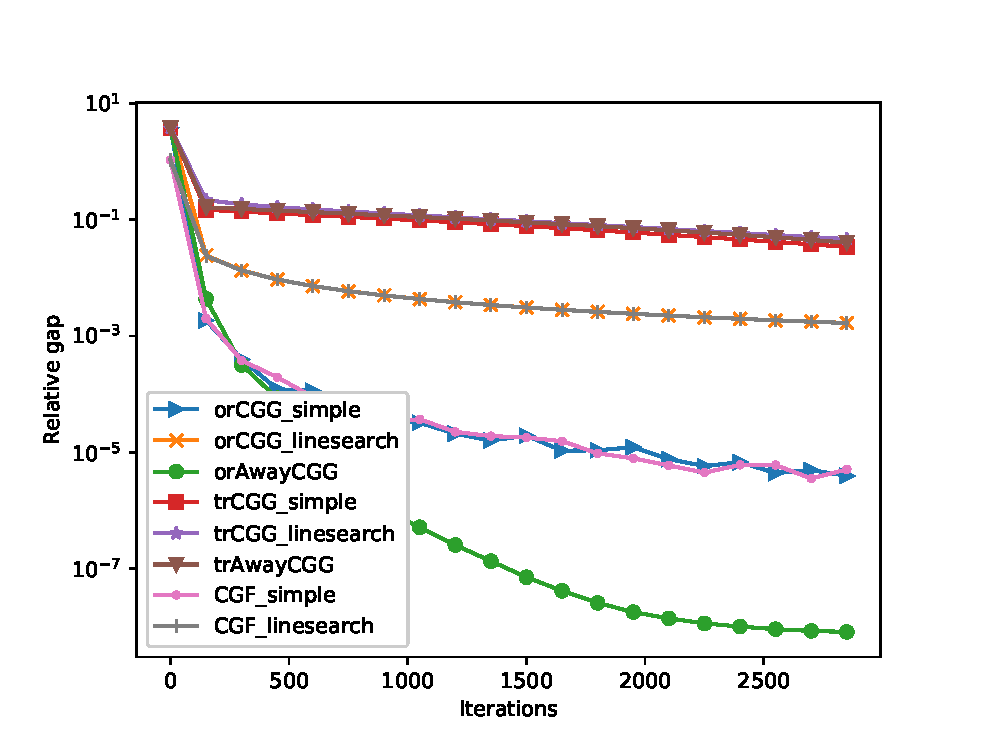
\includegraphics[height=7.2cm,width=9cm]{Images/Leastsquare_Iterations_vs_RelativeGap_5.eps}
	\caption{Iteration-Gap figure for trend filtering with quadratic loss $\| Ax-b\|^2$ and constraint $\|D^{(r)}\| \le \delta$, where $A\in \R^{N\times n}$, $r=1$, $N=200$, $n=400$ and $\delta= 0.8$. b is generated by $b = A\bar x +\epsilon$ with $\bar x$ being piecewise contant with 5 pieces and $\|D^{(1)} \bar x\|_1 = 1$. $\epsilon \sim N(0, \sigma^2)$ with noise $\sigma= 0.2 \|A\bar x\|_2 / \sqrt{N}$.   }
	\label{Iteration-Gap5}
\end{figure}


\begin{figure}[htbp]
	\centering
	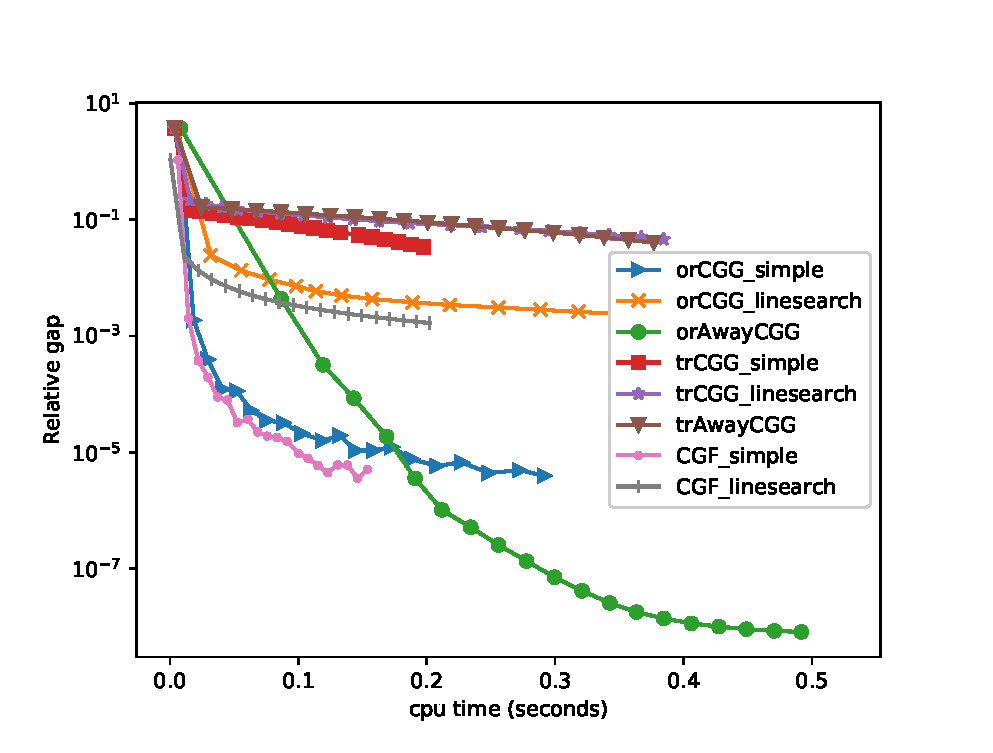
\includegraphics[height=7.2cm,width=9cm]{Images/Leastsquare_Time_vs_RelativeGap_5.eps}
	\caption{Time-Gap figure for trend filtering with quadratic loss $\| Ax-b\|^2$ and constraint $\|D^{(r)}\| \le \delta$, where $A\in \R^{N\times n}$, $r=1$, $N=200$, $n=400$ and $\delta= 0.8$. b is generated by $b = A\bar x +\epsilon$ with $\bar x$ being piecewise contant with 5 pieces and $\|D^{(1)} \bar x\|_1 = 1$. $\epsilon \sim N(0, \sigma^2)$ with noise $\sigma= 0.2 \|A\bar x\|_2 / \sqrt{N}$. The time taken by CVXPY is 0.406204 seconds. }
	\label{Time-Gap5}
\end{figure}





\begin{figure}[htbp]
	\centering
	\includegraphics[height=7.2cm,width=9cm]{Images/Logistic_Iterations_vs_RelativeGap_99.eps}
	\caption{Iteration-Gap figure for trend filtering with logistic loss $\sum_{i=1}^N \log \left( 1+\exp(-y_i\sigma x_i^T \beta) \right)$ and constraint $\|D^{(r)} \beta\|_1 \le \delta$, where $\beta\in \R^n$ with $N= 200$, $n = 400$, $r = 2$, $\delta= 0.8$ and $\sigma= 2.0e-02$. $y_1,...,y_N$ are i.i.d. samples generated from the distribution $\mathbb{P}(y_i = 1) = \frac{1}{1+\exp(-\sigma x_i^T \bar \beta)}, $ $\mathbb{P}(y_i = -1) = 1- \mathbb{P}(y_i = 1)$, where $\bar \beta$ is piecewise linear with 5 pieces and $\|D^{(r)} \bar \beta\|_1 = 1$.}
	\label{Iteration-Gap99}
\end{figure}


\begin{figure}[htbp]
	\centering
	\includegraphics[height=7.2cm,width=9cm]{Images/Logistic_Time_vs_RelativeGap_99.eps}
	\caption{Time-Gap figure for trend filtering with logistic loss $\sum_{i=1}^N \log \left( 1+\exp(-y_i\sigma x_i^T \beta) \right)$ and constraint $\|D^{(r)} \beta\|_1 \le \delta$, where $\beta\in \R^n$ with $N= 200$, $n = 400$, $r = 2$, $\delta= 0.8$ and $\sigma= 2.0e-02$. $y_1,...,y_N$ are i.i.d. samples generated from the distribution $\mathbb{P}(y_i = 1) = \frac{1}{1+\exp(-\sigma x_i^T \bar \beta)}, $ $\mathbb{P}(y_i = -1) = 1- \mathbb{P}(y_i = 1)$, where $\bar \beta$ is piecewise linear with 5 pieces and $\|D^{(r)} \bar \beta\|_1 = 1$. The time taken by CVXPY is 0.273652 seconds.}
	\label{Time-Gap99}
\end{figure}




\section{Least square fixed tolerance}

\begin{table}[H]
	\centering
	\label{Table_exp1}
	\begin{tabular}{cccc}
		\toprule
		{} &  CGG\_simple &  Awaystep\_CGG &  Mosek \\
		\midrule
		r=1, (N,n)=(500,50000), delta=0.8, sigma=0.5  &       7.987 &        15.838 & 75.009 \\
		r=1, (N,n)=(500,50000), delta=0.8, sigma=1.0  &       4.641 &         8.075 & 75.070 \\
		r=1, (N,n)=(500,50000), delta=1.2, sigma=0.5  &       9.205 &        16.263 & 77.466 \\
		r=1, (N,n)=(500,50000), delta=1.2, sigma=1.0  &       5.335 &         9.884 & 73.040 \\
		r=1, (N,n)=(5000,5000), delta=0.8, sigma=0.5  &       1.511 &         1.929 & 65.904 \\
		r=1, (N,n)=(5000,5000), delta=0.8, sigma=1.0  &       1.469 &         1.519 & 61.840 \\
		r=1, (N,n)=(5000,5000), delta=1.2, sigma=0.5  &       1.763 &         2.164 & 62.684 \\
		r=1, (N,n)=(5000,5000), delta=1.2, sigma=1.0  &       1.540 &         1.561 & 61.751 \\
		r=1, (N,n)=(10000,1000), delta=0.8, sigma=0.5 &       0.212 &         0.181 & 15.534 \\
		r=1, (N,n)=(10000,1000), delta=0.8, sigma=1.0 &       0.179 &         0.153 & 14.937 \\
		r=1, (N,n)=(10000,1000), delta=1.2, sigma=0.5 &       0.524 &         0.328 & 14.943 \\
		r=1, (N,n)=(10000,1000), delta=1.2, sigma=1.0 &       0.238 &         0.203 & 15.082 \\
		\bottomrule
	\end{tabular}
	\caption{Experiment1 on trend filtering with quadratic loss: The CPU time of CGG with simple step size and Awaystep-CGGto reach a fixed tolerance 1.0e-04 of the relative gap. The fourth column reports the time required by Mosek. All the reported results are the average of 3 independent experiments. The value -1 means that in at least one of the 3 experiments, the algorithm doesnot reach the tolerance 1.0e-04 within 10000 iterations}
\end{table}


\begin{table}[H]\
	\centering
	\label{Table_exp1}
	\begin{tabular}{cccc}
		\toprule
		{} &  CGG\_simple &  Awaystep\_CGG &  Mosek \\
		\midrule
		r=2, (N,n)=(500,30000), delta=0.8, sigma=0.5  &      -1.000 &        -1.000 & 38.810 \\
		r=2, (N,n)=(500,30000), delta=0.8, sigma=1.0  &      -1.000 &        -1.000 & 36.912 \\
		r=2, (N,n)=(500,30000), delta=1.2, sigma=0.5  &       6.678 &        13.012 & 38.652 \\
		r=2, (N,n)=(500,30000), delta=1.2, sigma=1.0  &       3.195 &         7.448 & 40.021 \\
		r=2, (N,n)=(5000,5000), delta=0.8, sigma=0.5  &       1.614 &         2.579 & 49.877 \\
		r=2, (N,n)=(5000,5000), delta=0.8, sigma=1.0  &       1.506 &         1.907 & 54.804 \\
		r=2, (N,n)=(5000,5000), delta=1.2, sigma=0.5  &       2.399 &        -1.000 & 39.903 \\
		r=2, (N,n)=(5000,5000), delta=1.2, sigma=1.0  &       1.777 &         2.520 & 38.715 \\
		r=2, (N,n)=(10000,1000), delta=0.8, sigma=0.5 &       0.337 &         1.782 & 11.265 \\
		r=2, (N,n)=(10000,1000), delta=0.8, sigma=1.0 &       0.234 &         0.428 & 11.263 \\
		r=2, (N,n)=(10000,1000), delta=1.2, sigma=0.5 &       1.549 &         4.056 & 11.174 \\
		r=2, (N,n)=(10000,1000), delta=1.2, sigma=1.0 &       0.468 &         1.004 & 11.137 \\
		\bottomrule
	\end{tabular}
	\caption{Experiment1 on trend filtering with quadratic loss: The CPU time of CGG with simple step size and Awaystep-CGGto reach a fixed tolerance 1.0e-04 of the relative gap. The fourth column reports the time required by Mosek. All the reported results are the average of 3 independent experimentsThe value -1 means that in at least one of the 3 experiments, the algorithm doesnot reach the tolerance 1.0e-04 within 10000 iterations}
\end{table}



\begin{table}[H]
	\centering
	\label{Table_exp1}
	\begin{tabular}{lrrr}
		\toprule
		{} &  CGG\_simple &  Awaystep\_CGG &  Mosek \\
		\midrule
		r=2, (N,n)=(500,20000), delta=0.8, sigma=0.5  &      -1.000 &        -1.000 & 24.666 \\
		r=2, (N,n)=(500,20000), delta=0.8, sigma=1.0  &       1.171 &         1.316 & 23.448 \\
		r=2, (N,n)=(500,20000), delta=1.2, sigma=0.5  &       2.295 &         3.669 & 24.865 \\
		r=2, (N,n)=(500,20000), delta=1.2, sigma=1.0  &       1.547 &         1.722 & 24.230 \\
		r=2, (N,n)=(5000,5000), delta=0.8, sigma=0.5  &       1.429 &         1.664 & 58.800 \\
		r=2, (N,n)=(5000,5000), delta=0.8, sigma=1.0  &       1.409 &         1.418 & 53.611 \\
		r=2, (N,n)=(5000,5000), delta=1.2, sigma=0.5  &       1.752 &         2.112 & 38.990 \\
		r=2, (N,n)=(5000,5000), delta=1.2, sigma=1.0  &       1.505 &         1.547 & 39.576 \\
		r=2, (N,n)=(10000,1000), delta=0.8, sigma=0.5 &       0.228 &         0.373 & 11.588 \\
		r=2, (N,n)=(10000,1000), delta=0.8, sigma=1.0 &       0.192 &         0.183 & 11.395 \\
		r=2, (N,n)=(10000,1000), delta=1.2, sigma=0.5 &       0.354 &         0.493 & 11.089 \\
		r=2, (N,n)=(10000,1000), delta=1.2, sigma=1.0 &       0.245 &         0.236 & 11.017 \\
		\bottomrule
	\end{tabular}
	\caption{Experiment1 on trend filtering with quadratic loss: The CPU time of CGG with simple step size and Awaystep-CGGto reach a fixed tolerance 5.0e-04 of the relative gap. The fourth column reports the time required by Mosek. All the reported results are the average of 3 independent experimentsThe value -1 means that in at least one of the 3 experiments, the algorithm doesnot reach the tolerance 5.0e-04 within 10000 iterations}
\end{table}



\section{Losigtic path}

\begin{table}[H]
	\centering
	\label{Table_logistic_path}
	\begin{tabular}{ccc}
		\toprule
		{} &  CGG\_simple &   CVXPY \\
		\midrule
		r=1, (N,n)=(200,2000), sigma=1.000e-04  &       0.505 & 145.772 \\
		r=1, (N,n)=(200,2000), sigma=2.500e-04  &       0.897 & 135.875 \\
		r=1, (N,n)=(3000,300), sigma=6.667e-04  &       0.031 & 294.511 \\
		r=1, (N,n)=(3000,300), sigma=1.667e-03  &       0.089 & 296.874 \\
		r=1, (N,n)=(1000,1000), sigma=2.000e-04 &       0.117 & 567.477 \\
		r=1, (N,n)=(1000,1000), sigma=5.000e-04 &       0.071 & 600.719 \\
		\bottomrule
	\end{tabular}
	\caption{Logistic path, tolerance = $1e-4$}
\end{table}



\begin{table}[H]
	\centering
	\label{Table_logistic_path}
	\begin{tabular}{ccc}
		\toprule
		{} &  CGG\_simple &   CVXPY \\
		\midrule
		r=2, (N,n)=(200,2000), sigma=1.000e-04  &      24.039 & 162.915 \\
		r=2, (N,n)=(200,2000), sigma=2.500e-04  &      58.720 & 163.414 \\
		r=2, (N,n)=(3000,300), sigma=6.667e-04  &       9.606 & 316.001 \\
		r=2, (N,n)=(3000,300), sigma=1.667e-03  &      28.916 & 409.973 \\
		r=2, (N,n)=(1000,1000), sigma=2.000e-04 &      31.361 & 402.629 \\
		r=2, (N,n)=(1000,1000), sigma=5.000e-04 &      71.114 & 463.311 \\
		\bottomrule
	\end{tabular}
	\caption{Logistic path, tolerance = $1e-4$}
\end{table}


\section{Matrix completion with side information}


\begin{table}[H] 
	\centering
	\label{MC-side-information}
	\begin{tabular}{ccccccc}
		\toprule
		(nnzr, snr, relative delta) &scs time &scs training error &scs test error &CGG time &CGG training error &CGG test error\\ 
		\midrule 
		(0.1, 3.0, 0.8)& 150.257  &0.060  &0.358  &9.480  &0.061  &0.369 \\ 
		(0.3, 3.0, 0.8)& 87.767  &0.118  &0.070  &2.007  &0.120  &0.074 \\ 
		(0.5, 3.0, 0.8)& 61.042  &0.124  &0.057  &1.191  &0.126  &0.060 \\ 
		(0.1, 1.0, 0.8)& 83.303  &0.233  &1.077  &3.559  &0.237  &1.075 \\ 
		(0.3, 1.0, 0.8)& 54.052  &0.424  &0.322  &1.377  &0.433  &0.333 \\ 
		(0.5, 1.0, 0.8)& 44.066  &0.472  &0.190  &0.796  &0.481  &0.201 \\ 
		(0.1, 3.0, 1.2)& 350.017  &0.000  &0.380  &-1.000  &0.000  &0.384 \\ 
		(0.3, 3.0, 1.2)& 145.559  &0.039  &0.050  &15.353  &0.039  &0.051 \\ 
		(0.5, 3.0, 1.2)& 87.267  &0.057  &0.027  &11.218  &0.058  &0.028 \\ 
		(0.1, 1.0, 1.2)& 119.298  &0.087  &1.103  &16.893  &0.089  &1.099 \\ 
		(0.3, 1.0, 1.2)& 65.107  &0.298  &0.329  &3.746  &0.304  &0.333 \\ 
		(0.5, 1.0, 1.2)& 53.793  &0.365  &0.190  &2.958  &0.373  &0.199 \\ 
		\bottomrule
	\end{tabular}
	\caption{Experiment on a problem with m = 300, n = 300, r = 5, r1 = 5, tol = 1.0e-02. The CGG time takes value -1 means it doesnot reach the 1.0e-02 tolerance within 10000 iterations.}
\end{table}

\begin{table}[H] 
	\centering
	\label{MC-side-information}
	\begin{tabular}{ccccccc}
		\toprule
		(nnzr, snr, relative delta) &scs time &scs training error &scs test error &CGG time &CGG training error &CGG test error\\ 
		\midrule 
		(0.1, 3.0, 0.8)& 150.535  &0.060  &0.358  &67.752  &0.060  &0.362 \\ 
		(0.3, 3.0, 0.8)& 87.103  &0.118  &0.070  &7.615  &0.118  &0.070 \\ 
		(0.5, 3.0, 0.8)& 60.423  &0.124  &0.057  &4.409  &0.124  &0.057 \\ 
		(0.1, 1.0, 0.8)& 84.064  &0.233  &1.077  &30.145  &0.233  &1.078 \\ 
		(0.3, 1.0, 0.8)& 54.346  &0.424  &0.322  &5.811  &0.425  &0.325 \\ 
		(0.5, 1.0, 0.8)& 44.276  &0.472  &0.190  &2.926  &0.473  &0.194 \\ 
		(0.1, 3.0, 1.2)& 360.665  &0.000  &0.380  &-1.000  &0.000  &0.384 \\ 
		(0.3, 3.0, 1.2)& 145.743  &0.039  &0.050  &92.647  &0.039  &0.050 \\ 
		(0.5, 3.0, 1.2)& 87.888  &0.057  &0.027  &58.179  &0.057  &0.027 \\ 
		(0.1, 1.0, 1.2)& 120.709  &0.087  &1.103  &131.111  &0.087  &1.102 \\ 
		(0.3, 1.0, 1.2)& 65.479  &0.298  &0.329  &18.689  &0.299  &0.330 \\ 
		(0.5, 1.0, 1.2)& 54.005  &0.365  &0.190  &13.179  &0.366  &0.191 \\ 
		\bottomrule
	\end{tabular}
	\caption{Experiment on a problem with m = 300, n = 300, r = 5, r1 = 5, tol = 1.0e-03. The CGG time takes value -1 means it doesnot reach the 1.0e-03 tolerance within 10000 iterations.}
\end{table}

%
\begin{table}[H] 
	\centering
	\label{MC-side-information}
	\begin{tabular}{ccccccc}
		\toprule
		(nnzr, snr, relative delta) &scs time &scs training error &scs test error &CGG time &CGG training error &CGG test error\\ 
		\midrule 
		(0.1, 3.0, 0.8)& 191.413  &0.060  &0.358  &500.576  &0.060  &0.359 \\ 
		(0.3, 3.0, 0.8)& 111.689  &0.118  &0.070  &31.818  &0.118  &0.070 \\ 
		(0.5, 3.0, 0.8)& 77.384  &0.124  &0.057  &16.837  &0.124  &0.057 \\ 
		(0.1, 1.0, 0.8)& 105.793  &0.233  &1.077  &198.904  &0.233  &1.077 \\ 
		(0.3, 1.0, 0.8)& 69.040  &0.424  &0.322  &30.496  &0.424  &0.323 \\ 
		(0.5, 1.0, 0.8)& 55.959  &0.472  &0.190  &13.548  &0.472  &0.191 \\ 
		(0.1, 3.0, 1.2)& 449.391  &0.000  &0.380  &-1.000  &0.000  &0.384 \\ 
		(0.3, 3.0, 1.2)& 176.350  &0.039  &0.050  &-1.000  &0.039  &0.050 \\ 
		(0.5, 3.0, 1.2)& 102.297  &0.057  &0.027  &327.819  &0.057  &0.027 \\ 
		(0.1, 1.0, 1.2)& 146.972  &0.087  &1.103  &-1.000  &0.087  &1.103 \\ 
		(0.3, 1.0, 1.2)& 81.549  &0.298  &0.329  &113.076  &0.298  &0.329 \\ 
		(0.5, 1.0, 1.2)& 67.093  &0.365  &0.190  &68.780  &0.365  &0.190 \\ 
		\bottomrule
	\end{tabular}
	\caption{Experiment on a problem with m = 300, n = 300, r = 5, r1 = 5, tol = 1.0e-04. The CGG time takes value -1 means it doesnot reach the 1.0e-04 tolerance within 10000 iterations.}
\end{table}




\bibliography{mybib_FW_unbounded_cons}
\bibliographystyle{plain}

\end{document}